\documentclass[12pt]{article}
\usepackage{amsmath}
\usepackage{amsthm}
\usepackage{algorithm}
\usepackage{algpseudocode}
\usepackage{amssymb}
\usepackage{graphicx}
\graphicspath{ {assets/} }

\begin{document}

\title{Assignment 2 - Quadtree and WSPD}
\author{
	Pattarawat Chormai - 0978675 \\
}
\maketitle

\section*{Q3}

\subsection*{a}

Let denote $h_1$ and $h_2$ lines define area of cone $C$ and $D_1$ and $D_2$
are vectors that pass the origin point and pendicular to $h_i$. The direction
of $D$ is defined by the face of $C$.

Denote $v(D_i,p)$ the value of point $p$ projected on $D_i$. We observe that for
all points $q \in C_p$, its $v(D_1,q)$ and $v(D_2,q)$ are greater than
the values of $p$, otherwise $q \notin C_p$, as shown in Figure $\ref{fig:theta-graph}$.

Thus, we shall use this property to develop a sweep line algorithm which works
as follows:

First, it intializes an event queue E by sorting $P$ in descending order of $v(D_1,p)$.
When processing $p_i$, the point will be added into a balanced binary search tree $S$, a status structure,
that has properties below :
\begin{itemize}
    \item An internal node $u$ store information related to searching.
    \item Points are stored in leaf level and sorted by $v(D_2,p)$ in ascending order.
    \item Node $u$ also stores $z_u$ which is the point $q$ from its right subtree whose $v(D_2,q)$ is lowest. \\
        \;\; Note that $z_u$ is updated during insertion process.
\end{itemize}

Next, the algorithm will traverse from the root of $S$ to the leaf of $p_i$. During traversal,
if the path go to left subtree of node $u$, then the algorithm will add $z_u$ in to an array $M$.
Then, the algorithm will find the lowest point for $C_{p_i}$ from $M$.

\begin{center}
    \label{figure1}
    \begin{figure}[h]
    \centering
    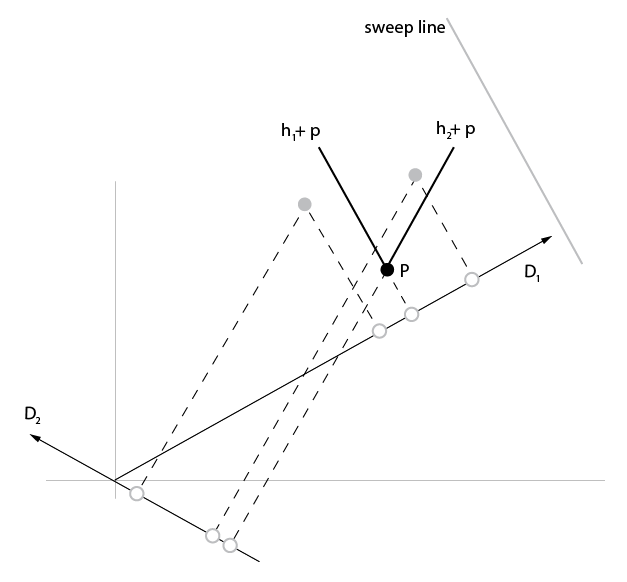
\includegraphics[width=10cm]{theta-graph}\\
    \caption{An example of how the algorithm works.} \label{fig:theta-graph}
    \end{figure}
\end{center}

\begin{algorithm}[h]
  \caption{OneConeGraph}
  \begin{algorithmic}
    \Require set of points $P$
    \State $E$ $\leftarrow$ Sort $p \in P$ using $v(D_1,p)$ in descending order.
    \State Intialize a status structure $S$.
    \State Intialize a set $G$
    \While{$E \neq \emptyset$}
        \State $p \leftarrow$ NextEvent(E)
        \State add $p$ into $S$
        \State $q \leftarrow$ FindClosestPoint(S, p)
        \State $G \leftarrow G \cup { (p,q) }$
    \EndWhile
    \State return $G$
  \end{algorithmic}
\end{algorithm}

\begin{algorithm}[h]
  \caption{FindClosestPoint}
  \begin{algorithmic}
    \State Intialize an empty array $M$
    \State $v \leftarrow$ root of $S$
    \While{ $v \neq p$}
        \If{ $p$ is in left subtree of $v$ }
            \State add $z_v$ into $M$
            \State $v \leftarrow$ left child of $v$
        \Else
            \State $v \leftarrow$ right child of $v$
        \EndIf
    \EndWhile
    \State return $q$ where $q_y = \min_{q \in M} (q_y)$
  \end{algorithmic}
\end{algorithm}

\subsection*{Correctness}
Based on the observation that a point $q \in C_p$ if and only if $v(D_1,q)$ and $v(D_2,q)$
are greater than $v(D_1,p)$ and $v(D_2,p)$ respectively. Assume $p$ is the point that 
is currently processed. Only points $q \in P$, whose $v(D_1,q)$ is greater than $v(D_1,p)$,
have been processed. Thus, no point $k \in S$ has $v(D1,k)$ lower than $v(D_1,p)$.

In $FindClosestPoint$, the algorithm traverses from the root of $S$ down to the leaf
of $p$. When passing an internal node $u$ and $p$ is in the left subtree of $u$,
the algorithm always adds $z_u$, the point in the right subtree of $u$  whose y-value is lowest, into $M$.

only points $q$ whose $v(D_2,q)$ is greater than $v(D_2,p)$. Hence, all points in $M$ is in $C_p$,
Thus, the point in $M$ whose lowest y-value is the lowest point in $C_p$ \\

\newpage
Therefore, $OneConeGraph$ will have the correct lowest point for all $p \in P$.

\subsection*{Running Time}
\begin{itemize}
    \item Construct $E$ takes $O(n\log{n})$.
    \item For processing each point, it takes \\
    $\;\;$ $O(1)$ for extracting the event.\\
    $\;\;$ $O(\log{n})$ for adding $p$ into $S$ and update $z_u$ if necessary. \\
    $\;\;$ $O(\log{n})$ for $FindClosestPoint$ because the size of $M$ is bounded by the depth of $S$. \\
\end{itemize}

Thus, the algorithm runs in $O(n\log{n})$ time.

\subsection*{b}
To construct $\theta$-graph of $P$, we will run $OneConeGraph$ for each cone. Thus,
we can compute $\theta$-graph of $P$ in $O(kn\log{n})$.

\end{document}
